Como se indica en el alcance del proyecto, el trabajo consta de cuatro etapas, análisis de requisitos y estudio previo, especificación, diseño e implementación y pruebas. 
Si tenemos en cuenta la fase de GEP, donde se realizo el análisis de requisitos y el estudio previo, que va del 14 de noviembre al 14 de septiembre de 2015, en la que se han estimado 20 horas de trabajo semanales lo que da un total de 80 horas.
La fase de especificación y diseño, que va del 15 de octubre al 14 de noviembre de 2015, en la que se ha estimado de la misma forma 20 horas de trabajo semanal, con lo que se estiman también 80 horas de trabajo.
En la fase de implementación donde se empieza a aplicar la metodologia ágil se ha dividido en 11 spints de dos semanas, a cada sprint se ha calculado un trabajo de 20 horas, menos en el ultimo que es más corto y se estiman 10, lo que da un total de 210 horas.
Finalmente para la revisión final de la documentación se estiman 20 horas cada semana.
En total se calcula que el trabajo tendrá un total de 410 horas de trabajo.
\newpage

\subsection{Gantt}
Dado que en el proyecto se desarrolla íntegramente por una sola persona, la secuencialidad del diagrama es absoluta.
\\ Durante la fase de desarrollo simplemente se especifican los \textit{Sprints} que se llevaran a cabo hasta conseguir la consecución del proyecto, a medida que las historias de usuario se vayan redactando y priorizando se irán asignando a los \textit{sprints}.

\subsubsection{Tareas y Gráficos gantt}
\begin{figure}[ht!]
\center
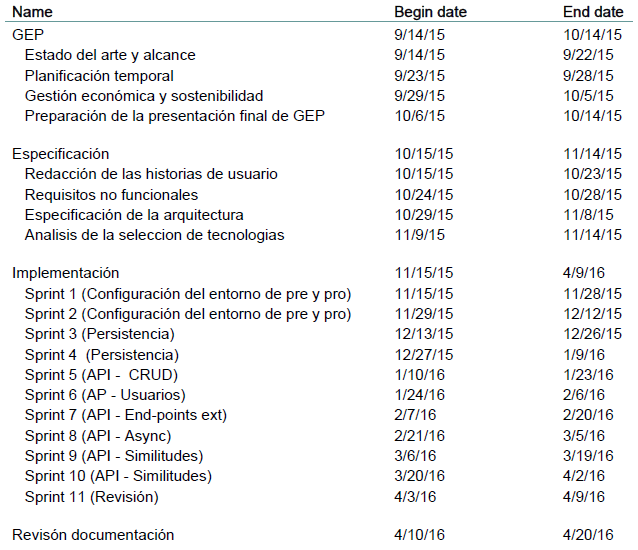
\includegraphics[scale=0.7]{Task.png}
\caption{Tareas del diagrama de gantt.}
\label{fig:task}
\end{figure}
\newpage
\begin{landscape}
\begin{figure}[ht!]
\center
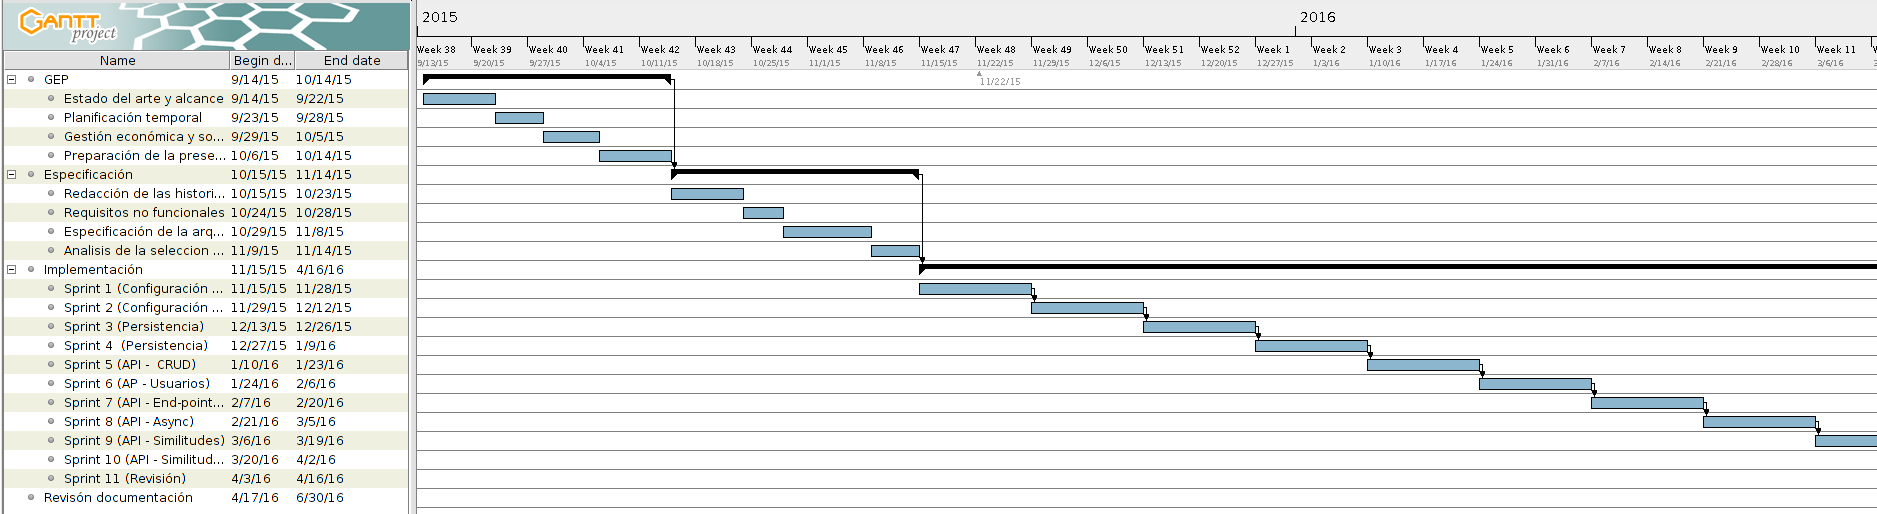
\includegraphics[width=\textwidth,height=\textheight,keepaspectratio]{Gantt_1.PNG}
\caption{Diagrama de gantt.}
\label{fig:gantt_1}
\end{figure}

\begin{figure}[ht!]
\center
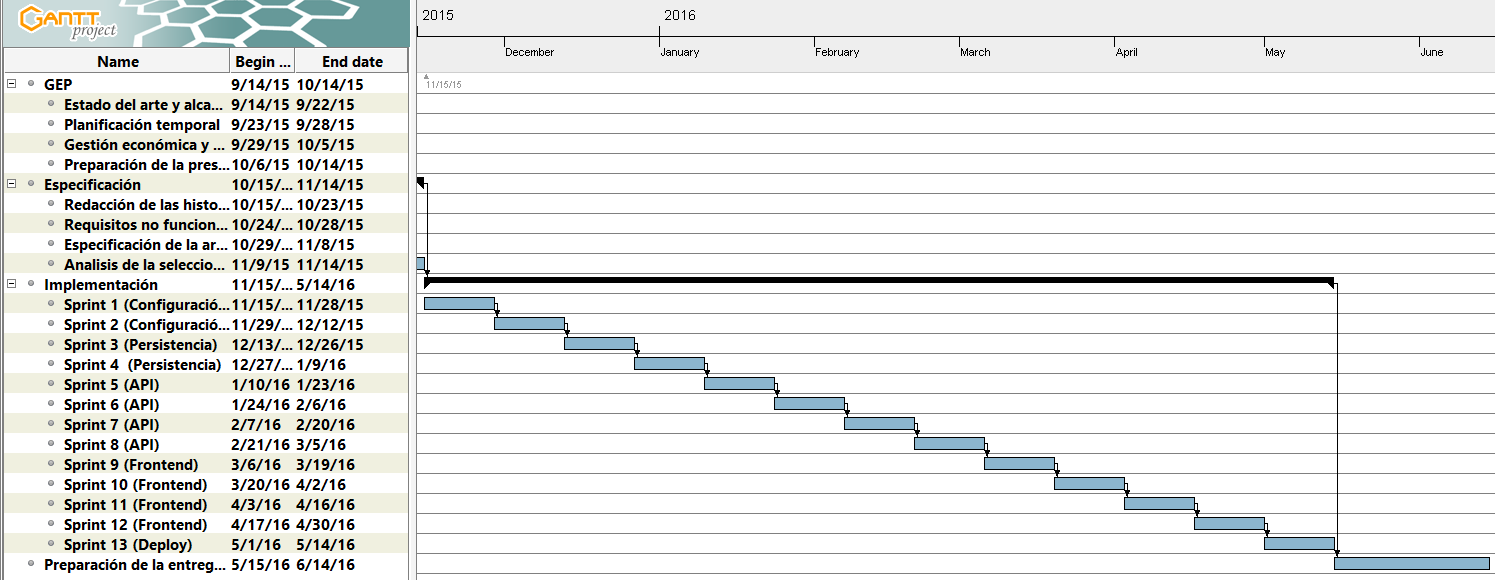
\includegraphics[width=\textwidth,height=\textheight,keepaspectratio]{Gantt_2.PNG}
\caption{Diagrama de gantt.}
\label{fig:gantt_2}
\end{figure}

\end{landscape}
\newpage

\subsection{Recursos}
Las necesidades en recursos serán muy escuetas dado que todo el software que se usara es libre y las maquinas en las que se trabaja en pre-producción serán virtuales. La única necesidad de tener unos recursos que se necesiten planificar, ya que requieren ser contratados, son los servidores en los que se hará el \textit{deploy}, se tendrán que contratar durante las semanas que dures los \textit{sprints} en los que se haga el \textit{deploy.} Por otro lado en cuanto a recursos humanos el proyecto se llevara a cabo por un solo desarrollador que se encargar tanto de la programación como la documentación.

\subsection{Alterativas y plan de acción}
Dado que el proyecto se desarrollara usando \textit{Scrum}, al final de cada \textit{sprint}, durante el \textit{sprint backlog} se determinara si se han cumplido las expectativas del \textit{sprint}. Por otro lado en el \textit{sprint planning} se tendrá en cuenta si han habido carencias o \textit{bugs} en los anteriores \textit{sprints} para incorporarlos como historias de usuario al siguiente \textit{sprint}. 

Como se ha comentado en el alcance, se diseñara un software abierto orientado al desarrollo continuado. Por lo que en el \textit{sprint} 11 se dará por concluido el proyecto, y se documentara el estado en el que se encuentre y las historias de usuario pendientes, así como las desviaciones de la planificación inicial. 
\newpage
